\documentclass[reprint,english,notitlepage]{revtex4-2}  % defines the basic parameters of the document

% if you want a single-column, remove reprint

% allows special characters (including æøå)
\usepackage[utf8]{inputenc}
\usepackage[english]{babel}

%% note that you may need to download some of these packages manually, it depends on your setup.
%% I recommend downloading TeXMaker, because it includes a large library of the most common packages.

\usepackage{physics,amssymb}  % mathematical symbols (physics imports amsmath)
\usepackage{graphicx}         % include graphics such as plots
\usepackage{xcolor}           % set colors
\usepackage{hyperref}         % automagic cross-referencing (this is GODLIKE)
\usepackage{tikz}             % draw figures manually
\usepackage{listings}         % display code
\usepackage{subfigure}        % imports a lot of cool and useful figure commands

% defines the color of hyperref objects
% Blending two colors:  blue!80!black  =  80% blue and 20% black
\hypersetup{ % this is just my personal choice, feel free to change things
    colorlinks,
    linkcolor={red!50!black},
    citecolor={blue!50!black},
    urlcolor={blue!80!black}}

%% Defines the style of the programming listing
%% This is actually my personal template, go ahead and change stuff if you want
\lstset{ %
	inputpath=,
	backgroundcolor=\color{white!88!black},
	basicstyle={\ttfamily\scriptsize},
	commentstyle=\color{magenta},
	language=Python,
	morekeywords={True,False},
	tabsize=4,
	stringstyle=\color{green!55!black},
	frame=single,
	keywordstyle=\color{blue},
	showstringspaces=false,
	columns=fullflexible,
	keepspaces=true}


%% USEFUL LINKS:
%%
%%   UiO LaTeX guides:        https://www.mn.uio.no/ifi/tjenester/it/hjelp/latex/
%%   mathematics:             https://en.wikibooks.org/wiki/LaTeX/Mathematics

%%   PHYSICS !                https://mirror.hmc.edu/ctan/macros/latex/contrib/physics/physics.pdf

%%   the basics of Tikz:       https://en.wikibooks.org/wiki/LaTeX/PGF/TikZ
%%   all the colors!:          https://en.wikibooks.org/wiki/LaTeX/Colors
%%   how to draw tables:       https://en.wikibooks.org/wiki/LaTeX/Tables
%%   code listing styles:      https://en.wikibooks.org/wiki/LaTeX/Source_Code_Listings
%%   \includegraphics          https://en.wikibooks.org/wiki/LaTeX/Importing_Graphics
%%   learn more about figures  https://en.wikibooks.org/wiki/LaTeX/Floats,_Figures_and_Captions
%%   automagic bibliography:   https://en.wikibooks.org/wiki/LaTeX/Bibliography_Management  (this one is kinda difficult the first time)
%%   REVTeX Guide:             http://www.physics.csbsju.edu/370/papers/Journal_Style_Manuals/auguide4-1.pdf
%%
%%   (this document is of class "revtex4-1", the REVTeX Guide explains how the class works)


%% CREATING THE .pdf FILE USING LINUX IN THE TERMINAL
%%
%% [terminal]$ pdflatex template.tex
%%
%% Run the command twice, always.
%% If you want to use \footnote, you need to run these commands (IN THIS SPECIFIC ORDER)
%%
%% [terminal]$ pdflatex template.tex
%% [terminal]$ bibtex template
%% [terminal]$ pdflatex template.tex
%% [terminal]$ pdflatex template.tex
%%
%% Don't ask me why, I don't know.

\begin{document}
\title{This is a Very Important Title!}   % self-explanatory
\author{Person McSomething}               % self-explanatory
\date{\today}                             % self-explanatory
\noaffiliation                            % ignore this
\begin{abstract}                          % marks the beginning of the abstract
This abstract is abstract.                % the body of the abstract
\end{abstract}                            % marks the end of the abstract
\maketitle                                % creates the title, author, date & abstract

If you want to learn more about using \LaTeX, you should check UiO's official tutorials:
\url{https://www.mn.uio.no/ifi/tjenester/it/hjelp/latex/}

If you are familiar with \LaTeX\ and you want to learn more about the REVTeX4-1 document class, check:
\url{http://www.physics.csbsju.edu/370/papers/Journal_Style_Manuals/auguide4-1.pdf}


% the fundamental components of scientific reports:
\section{Introduction}


\section{Theory}   % (optional)
\section{Method}

\section{Results}
\section{Discussion}
\section{Conclusion}
% acknowledgements (optional)
\begin{acknowledgments}  % if you disagree with the spelling, blame Americans
I would like thank myself for writing this beautiful document.
\end{acknowledgments}


%% When it comes to the bibliography I personally generate it using BibLaTeX. (see the link above if you're interested)
%% You're obviously allowed to create the references section however you like.
%% I'll keep it simple here.
\section*{References}  % the asterisk (*) after \section makes the section numbering go away
\begin{itemize}
\item[-]Reference 1
\item[-]Reference 2
\end{itemize}

\newpage
%% if you want to include an appendix, this is how you do it
\appendix
\section{Name of appendix}
This will be the body of the appendix.
\section{This is another appendix}\label{appendix}
Tada.
%% all \section commands following \appendix are automatically taken as appendices

%% Note that \label{appendix} command on line 115. What this does is setup a reference point for LaTeX that you can
%% access wherever you want using \ref{appendix}.
%% You can place labels on most environments such as equations, figures, tables, etc.

\clearpage
Note that this document is written in the two-column format. If you want to display a large equation, a large figure, or whatever, in one-column format, you can do this like so:
\onecolumngrid
\vspace{1cm} % some extra space
This text and this equation are both in one-column format.

\footnote{This equation is actually from quantum mechanics. ``It's called Schrödinger's Time-Dependent Wave Equation'', named after the awesome Austrian physicist Erwin Rudolf Josef Alexander Schrödinger. Yep, the ``Schrödinger's cat'' guy. Pretty cool dude actually, check his wiki page: \url{https://en.wikipedia.org/wiki/Erwin_Schrodinger}. He was physics' no. 1 Ladies' man if there ever was one. Anyway, you will learn more about this equation in FYS2140. You can also find it printed on a glass wall in the UiO Physics Building (it really is that important).}

\begin{equation}\label{equation}
\frac{-\hbar^2}{2m}\laplacian{\Psi}+V\Psi=i\hbar\pdv{t}\Psi
\end{equation}
Note that the equation numbering (this: \ref{equation}) follows the appendix as this text is technically inside Appendix \ref{appendix}. If you want a detailed listing of (almost) every available math command, check: \url{https://en.wikibooks.org/wiki/LaTeX/Mathematics}.
\vspace{1cm} % some extra space
\twocolumngrid
And now we're back to two-column format. It's really easy to switch between the two. It's recommended to keep the two-column format, because it is easier to read, it's not very cluttered, etc. Pro Tip: You should also get used to working with REVTeX because it is really helpful in FYS2150.

One last thing, this is a code listing:
\begin{lstlisting}
This will be displayed with a cool programming font!
\end{lstlisting}
You can add extra arguments using optional parameters:
\begin{lstlisting}[morekeywords={cool}]
This will be displayed with a cool programming font!
\end{lstlisting}
You can also list code from a file using \texttt{lstinputlisting}. If you're interested, check \url{https://en.wikibooks.org/wiki/LaTeX/Source_Code_Listings}.

This is a basic table:
\begin{table}[h]  % h = "here"  , h! = here!
\caption{This is a nice table}\label{table}
\begin{tabular}{|c|c|c|} % note that & separates columns while \\ separates the rows
\hline                    % creates a horizontal line (try removing it)
Hey & Hey & Hey  \\
\hline
Hello & Hello & Hello \\
\hline
Bye & Bye & Bye \\
\hline
\end{tabular}
\end{table}\\
You can a detailed description of tables here: \url{https://en.wikibooks.org/wiki/LaTeX/Tables}.

This is a more advanced table:
%tabell i latex
\begin{table}[h!] %%h! er for å tvinge tabellen til å være nærmest mulig her i dokumentet
  \begin{center}
    \caption{Tabelleksempel} %Tabelltekst
    \label{tab:results}
    \begin{tabular}{l|c|r} % for hver kolonne har du {a|b|c} der a er for 1.kolonne, b for 2. kolonne etc, l=venstrestil, r=høyrestilt, c = senterstilt. Se posisjonen til tallene i de forskjellige kolonnene. Har du 4 kolonner der alle er senterstilt blir det f.eks. {c|c|c|c}
      \textbf{Partikkelindeks} & \textbf{Posisjon} & \textbf{Hastighet}\\ %innhold i hver kolonne, legg til flere her hvis du har flere kolonner
      (i) & (m) & (m/s)\\ %enheter for hver kolonne
      \hline %en horisontall linje for å skille overskriften fra tallene under. Vil du ha en slik linje mellom hver rad i tabellen så legg til en \hline mellom hver rad nedover her. Merk \\ er som vanlig linjeskift mens & skiller kolonner
      0 & 139.22 & 12.4\\
      1 & 14.88 & 18.7\\
      2 & 233.9 & 10.10\\
      3 & 816.12 & 13.4\\
      \hline
    \end{tabular}
  \end{center}
\end{table}



I'm not going to delve into Tikz in any level detail, but here's a quick picture:
\begin{figure}[h]
\centering  % places the tikz image in the center of the text column
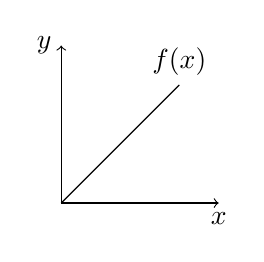
\begin{tikzpicture}
\draw[->] (0,0) -- (2,0) node [pos=1.0,below] {\(x\)};
\draw[->] (0,0) -- (0,2) node [pos=1.0,left] {\(y\)};
\draw (0,0) -- (1.5,1.5) node [pos=1.0,above] {\(f(x)\)};
\end{tikzpicture}
\caption{This is great caption}\label{figure}
\end{figure}\\
If you want to know more, check: \url{https://en.wikibooks.org/wiki/LaTeX/PGF/TikZ}.

%% If you want to include figure:
%\includegraphics[scale=1.0]{filename}
%% check https://en.wikibooks.org/wiki/LaTeX/Importing_Graphics if you want to know more

\end{document}
